\chapter{Describing Processes with Natural Language}
\label{cha:atd}

In this chapter, we describe the use case of Annotated Textual
Descriptions (ATD) in natural langauge to describe business processes.
Section~\ref{sec:atd_running_example} presents a process model example that will be
used throughout this document for illustrative purposes. Next,
Section~\ref{sec:atd_atd} contains a rationale for ATD. Finally,
Section~\ref{sec:atd_semantics} describes the semantics of the base ATD language.

\section{Running Example}
\label{sec:atd_running_example}

In order to provide an illustrative example for the remainder of this document,
let us consider a process of patient examination\footnote{Based on the
  description provided by the Women's Hospital of Ulm. Both the text and the
  model are extracted from~\cite{CabanillasKRRMC15}.}.  The textual description
of this process is provided in Figure~\ref{fig:running_example}. Additionally,
figure~\ref{fig:running_example_bpmn} shows the equivalent process model in a
well-known process notation: BPMN.

\begin{figure}
\centering
{%
\setlength{\fboxsep}{6pt}
\fbox{
\parbox{0.85\textwidth}{
\emph{
The examination process can be summarised as follows. The process starts
when the female patient is examined by an outpatient physician, who decides
whether she is healthy or needs to undertake an additional examination. In the
former case, the physician fills out the examination form and the patient can
leave. In the latter case, an examination and follow-up treatment order is placed
by the physician, who additionally fills out a request form. Beyond information
about the patient, the request form includes details about the examination 
requested and refers to a suitable lab. Furthermore, the outpatient physician
informs the patient about potential risks. If the patient signs an informed consent
and agrees to continue with the procedure, a delegate of the physician
arranges an appointment of the patient with one of the wards. The latter is
then responsible for taking a sample to be analysed in the lab later. Before the
appointment, the required examination and sampling is prepared by a nurse of
the ward based on the information provided by the outpatient section. Then, a
ward physician takes the sample requested. He further sends it to the lab indicated
in the request form and conducts the follow-up treatment of the patient.
After receiving the sample, a physician of the lab validates its state and decides
whether the sample can be used for analysis or whether it is contaminated and
a new sample is required. After the analysis is performed by a medical technical
assistant of the lab, a lab physician validates the results. Finally, a physician
from the outpatient department makes the diagnosis and prescribes the therapy
for the patient.
}}}}
\caption{\label{fig:running_example} Textual description of a patient examination process.}
\end{figure}

\begin{figure}[hbt]
  \centering
  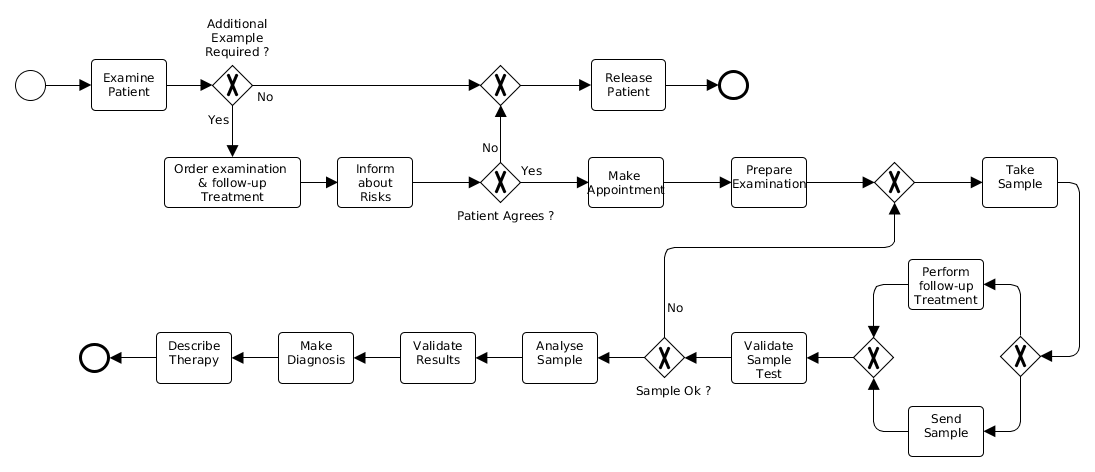
\includegraphics[width=0.8\textwidth]{figures/hospital}
  \caption{Process model for the patient examination process.}
  \label{fig:running_example_bpmn}
\end{figure}

\section{Annotated Textual Descriptions}
\label{sec:atd_atd}

In order to support the efficient creation and communication of business
processes, we must establish notation that is close to the mental framework of
all the actors involved in the process. Natural language is an ideal tool for
this task, being the clear winner in human communication.

%However, natural language alone suffers from ambiguity, and its unstructured
%nature makes automatic processing difficult and unreliable, despite all the
%recent advances in Natural Language Processing. 

However, using natural language alone has several drawbacks. Natural Language
Processing tools are getting increasingly better at extracting structure out of
plain text. However, some ambiguities remain an open issue to this day.
Furthermore, we argue that some of these issues cannot be automatically solved
reliably enough, since they require extensive domain knowledge. For instance, in
the example from  Figure~\ref{fig:running_example}, the sentence \emph{"The
  latter [physician] is then responsible for taking a sample to be analysed in
  the lab later"} highlights two important sources of ambiguity in the analysis
of textual descriptions: \emph{(i)} The action \emph{analyse} is described, but
it may not happen until later into the process, as hinted by the word
\emph{later}. Extracting this kind of temporal relationships from textual
descriptions is a very complex task~\cite{Mirza16}, with no good solutions in
the context of business processes. \emph{(ii)} Depending on the purpose of the
process, the same \emph{analyze} verb could actually be irrelevant from an
organizational point of view, if the {\em lab} were to be considered an external
entity. This presents an issue that cannot be solved without deep understanding
of the organization. In order to solve this, while still preserving the idea of
a flexible and natural way of describing processes, we rely on text annotations
(See Section~\ref{sec:background_anns}) as a common langauge to be used by
humans and computer systems.

We have named this new documentation format Annotated Textual Descriptions
(ATD). An ATD can be used as a replacement for any business process modeling
notation: A human reader can easily get a grasp of the process by simply reading
the text without the annotations, and can use the annotations to clarify any
ambiguities encountered (e.g. whether two activities can be executed
concurrently). On the other hand, a computer system can rely on the annotations
to automatically extract structure and additional semantic information from the
process, without the need to leverage a generic semantic graph\cite{PadroS12}.
The design goals of ATD can be summarized as follows:


\begin{description}
\item[Can Model Ambiguity] {Ambiguity is an inherent property of some processes.
    In some cases, an organization cannot reliably document every aspect of a
    business process. An example of this pehomena are error scenarios. Consider
    the sentence ``If everything is correct, the bank proceeds to charge the
    payment into the user's account''. This sentence is implicitly saying that,
    under some circumstances the execution will end in an undesired state if the
    bank cannot proceed with the payment. However, the phrasing clearly
    indicates that such error scenarios are outside the scope of the process. In
    cases like this, other techniques force the modeler to disambiguate the
    unclear parts of the process, resulting in too restrictive models that do
    not fully represent the reality of the organization. On the other hand, ATD
    are designed to capture the ambiguity by being built on an \emph{open
      world assumption}: If a part of the process is not clearly documented, we
    assume anything that happens is correct. This characterization of ambiguity
    also allows to automatically detect and report the ambiguous elements in
    order to improve the process.}
\item[Rich Semantics]{Since natural language is used as the main building block
    of ATD, any idea can be communicated with them. At the human level, the
    expressive power of the language is almost on par with the mental model of
    the writer. At the annotation level, ATD are designed to easily incorporate
    extensions into the annotations, so they can be adapted to multiple use
    cases. An example of that is seen in Chapter~\ref{cha:modeljudge}, where the
    base annotation language is expanded to enable automatic evaluation of
    students.}
\item[Low Representational Bias]{Representational bias is the phenomena where
    the notation being used forces the author of a process to model things in a
    certain way\cite{van2011representational}. For example, notations based on
    Petri Nets are well suited to model concurrency. However, there is no clear
    built-in mechanism to express the limits of iterative structures. This is
    why languages like BPMN have a built-in semantic element to model
    concurrency, the \emph{parallel gateway}, while loop conditions have to be
    expressed as text notes, which cannot be interpreted by computer systems.
    ATD, being close to the mental model of the actors involved in the process,
    have a low representational bias.}
\item[Automation]{To ensure adoption of a new language, ease of use is a very
    important factor to consider. Models must be easy to build and redundant
    constructs (i.e. \emph{boilerplate}) must be kept at a minimum. In ATD, the
    provided tooling ensures that such redundant tasks are automated: On one
    hand, an NLP tool generates an initial annotation for the user to refine,
    which typically just consists of removing unnecessary annotations. On the
    other hand, intuitive rules have been encoded in an inference engine to
    avoid unnecessary annotating. For example, the \emph{Coreference Relation}
    (See Section~\ref{sec:atd_relations}) is transitive and symmetric by
    default, saving redundant annotations. Similarly, the \emph{Sequential
      Relation} is added by default for two consecutive activities in the text
    if no other relation is specified.}
\end{description}



%- Present ATD as a PM notation
%- Characteristics
  %- Can model ambiguity (flexible)
  %- Open-world assumption: What's not explicit could be anything
  %- Little representational bias 
  %- Declarative 
  %- Rich semantics: Not only process flow
  
%- Requirements
  %- Must be able to represent everything that we need
  %- Ergonomics: Easy to annotate, no "boilerplate" (thanks to reasoning)
%
%- Motivate the need for annotations vs plain text:
  %- Some things cannot be inferred w/o domain knowledge
  %- NLP state-of-the-art can't accurately annotate text like we want to, this
  %intermediate step helps add structure, and also presents a format to create
  %future datasets.

\section{ATD Semantics}
\label{sec:atd_semantics}

ATD are designed to be adaptable. In this section, we describe the base language
which aims to represents the common concepts in all business processes.
Additionally, extensions are allowed in the form of new \emph{annotation} or
\emph{relation} specializations, to support more specific use cases. An example
of such expansion can be seen in Chapter~\ref{cha:modeljudge}.


%- Describe basic building blocks: Annotations, Relations
An ATD is defined as a set of annotations on top of a base text, written in
natural language. More formally, we can define an ATD as a $\langle T, A, R \rangle$ tuple, where 

%TODO: WIL: PRESENT AS BASE LANGUAGE + ARBITRARY EXTENSIONS

\begin{description}
\item{$\mathbf{T}$}{ is a string of characters representing the textual description.}
\item{$\mathbf{A}$}{ is a set of \emph{annotations}. Each annotation $\alpha =
    \langle type, start, end, \rangle$ marks a relevant aspect of the business
    process. The $start$ and $end$ integers mark the positions of a substring of
    T, and the $type$ is used to add semantics to the annotation. The types of
    annotations are defined as a hierarchy, so an annotation types can be specialized
    into subtypes.}
\item{$\mathbf{R}$}{ is a set of triples $\langle t, \alpha_i,
    \alpha_j \rangle$ representing binary relations of type $t$ between pairs of
    annotations $\alpha_i$, $\alpha_j$. Similarly, the $type$ of a relation is
    used to add particular semantics to it, and especialization of relation
    types is allowed.}
\end{description}

Next, we describe each of the annotation and relation types that we consider for
the base language of ATD. Table~\ref{tab:example_atd} shows an example of an
ATD which we will use for the remainder of this section.

\begin{table}[htb]
  \hspace*{-0.1\textwidth}
  \resizebox{1.2\textwidth}{!}{%
\begin{tabular}{r | c l}
& \textbf{Type} & \textbf{Start, End} \\
\bottomrule[1pt]
$\alpha_1$ & \emph{action} & ``an examination and follow-up treatment order is {\color{blue} \textbf{placed}} by the physician'' \\
\hline
$\alpha_2$ & \emph{action} &  ``is then responsible for taking a sample to be {\color{blue} \textbf{analysed}} in the lab'' \\
\hline
$\alpha_3$ & \emph{action} & ``After receiving the sample, a physician of the lab {\color{blue} \textbf{validates}} its state''  \\
\hline
$\alpha_4$ & \emph{role} & ``an examination and follow-up treatment order is placed by the {\color{blue} \textbf{physician}}'' \\
\hline
$\alpha_5$ & \emph{role} & ``the female patient is examined by an {\color{blue} \textbf{outpatient physician}}'' \\
\hline
$\alpha_6$ &  \emph{object} & ``an {\color{blue} \textbf{examination and follow-up treatment order}} is placed by the physician''\\
\hline
$\alpha_7$ &  \emph{condition} & ``decides whether {\color{blue} \textbf{she is healthy}} or needs to undertake additional examination''\\
\hline
$\alpha_8$ &  \emph{optional}, & ``the patient can {\color{blue} \textbf{leave}}''\\
&  \emph{ending} & \\
\hline
$\alpha_9$ &  \emph{implicit} & ``The patient is {\color{blue} \textbf{asked}} to sign an informed consent'' (Added text)\\
\hline
$\alpha_{10}$ &  \emph{action} & ``The required examination and sampling is {\color{blue} \textbf{prepared}} by a nurse'' \\
\hline
$\alpha_{11}$ &  \emph{action} & ``The required examination and sampling is {\color{blue} \textbf{prepared}} by a nurse''\\
\hline
$\alpha_{12}$ &  \emph{object} & ``The required {\color{blue} \textbf{examination}} and sampling is prepared by a nurse''\\
\hline
$\alpha_{13}$ &  \emph{object} & ``The required examination and {\color{blue} \textbf{sampling}} is prepared by a nurse''\\
\hline
$\alpha_{14}$ & \emph{role} & ``After receiving the sample, a {\color{blue} \textbf{physician}} of the lab validates its state''  \\
\toprule[1pt]
\end{tabular}
\hspace{0.1cm}
\begin{tabular}{r | c c c}
& \textbf{Type} & $\mathbf{\alpha_i}$ & $\mathbf{\alpha_j}$ \\
\bottomrule[1pt]
$r_1$ & \emph{agent} & $\alpha_1$ & $\alpha_4$ \\
\hline
$r_2$ & \emph{patient} & $\alpha_1$ & $\alpha_6$ \\
\hline
$r_3$ &  \emph{sequential} & $\alpha_2$ & $\alpha_3$ \\
\hline
$r_4$ &  \emph{coreference} & $\alpha_4$ & $\alpha_5$ \\
\hline
$r_5$ & \emph{patient} & $\alpha_{10}$ & $\alpha_{12}$ \\
\hline
$r_6$ & \emph{patient} & $\alpha_{11}$ & $\alpha_{13}$ \\
\hline
  $r_7$ &  \emph{fusionable} & $\alpha_{10}$ & $\alpha_{11}$ \\
\toprule[1pt]
\end{tabular}}
\caption{Example fragment of Annotated Textual Description with annotations (left) and relations (right).}
\label{tab:example_atd}
\end{table}


\subsection{Annotation Types}

Annotations are used to mark an important region of the text. In the base
language of ATD, we consider the following types of annotations which directly
map to some well-known concepts in the context of business processes.

\begin{description}
\item[Action.]{The \emph{action} annotation is used to represent the steps of the
    business process model, which are often associated with verbs. An example action
    would be \emph{placing} ($\alpha_1$) an examiation order. Each action
    corresponds to a single activity in the process model.}
\item[Entity.]{An anything that participates in the business process, either
    actively or passively. This is a generic type that is especialized in two
    subtypes: \emph{role} and \emph{business object}.}
\item[Role.]{A type of \emph{Entity}. The \emph{role} annotation is used to
    represent the autonomous actors involved in the process, like the
    \emph{outpatient physician} ($\alpha_5$). Any mention of an entity that
    performs some Action is considered a Role.}
\item[Business Object.]{The business object annotation is used to mark all the 
    relevant elements of the process that do not take an active part in it, such as 
    an \emph{examination order} ($\alpha_6$).
    In other notations, correspondences with business objects are typically
    found in activity labels and explicit elements such as data object references}
\item[Condition.]{A condition annotation indicates a part of the text that
    represents a pre-requisite for some part of the process being executed, such 
    as the patient \emph{being healthy} ($\alpha_7$). Conditions are typically 
    associated with XOR-splits, their labels and their surroundings.}
\end{description}

%- Action
  %- Optional
  %- ...
 %
%- Role
  %- Person
  %- Computer System?
%
%- Object
  %- Data Store
  %- ...
%- Condition / Event

\subsection{Relation Types}
\label{sec:atd_relations}

%- Agent, Patient
%- Coreferences
%- Control Flow

\begin{description}
\item[Agent.]{A \emph{role} is the \emph{agent} of an \emph{action} whenever the
    entity represented by the role performs that action. 
    %Using the example sentence  \emph{"an examination and follow-up treatment order is placed by the physician"}, the \emph{physician} is the \emph{agent} of \emph{placed}
    For instance, relation $r_1$ tells us it is the \emph{physician} who \emph{places} something.}
\item[Patient.]{An \emph{entity}, is the \emph{patient} of an \emph{action}
    whenever it acts as the recipient of the action. Relation $r_2$ tells us
    that what is \emph{placed} is an \emph{examination order}.}
\item[Control Flow.]{The \emph{sequential}, \emph{exclusive} and \emph{parallel}
    binary relationships, which are borrowed from behavioral
    profiles~\cite{smirnov2010business}, are used to indicate the order between \emph{action}s
    in the textual description. Due to the characteristics of natural language
    text, there is an open world assumption on the set of control flow
    relationships: Assuming an absence of contradictions, everything that is
    stated as relationship is enforced. However, no assumptions are made on
    things that are not specified. 
    In our example, \emph{analyse} ($\alpha_2$) is \emph{sequential} ($r_3$) --i.e. happens before--
    to \emph{validates} ($\alpha_3$)}
\item[Coreferences.]{An \emph{entity} is a coreference of another \emph{entity} when
    they refer to the same real world entity. The coreference relation forms a graph with
    one connected component per process entity. All ocurrences of the "patient" role in the
    example text are coreferences. However, there are two different "physician" 
    roles in the text, the "outpatient physician" ($\alpha_4$, $\alpha_5$) and the 
    "physician of the lab" ($\alpha_{14}$), which form two disconnected coreference graphs.}
\item[Fusionable Actions.]{Some \emph{actions} can be expressed at multiple
    granularity levels depending on the context. When two actions are
    fusionable, it means they can be represented as a single one without
    changing the semantics of the process. In the sentence \emph{"the required examination 
    and sampling is prepared"}, we could assume two independent actions \emph{prepare 
    (examination)} ($\alpha_{10}$) and \emph{prepare (sampling)} ($\alpha_{11}$) or a single 
    one \emph{prepare (examination  and sampling)}, as indicated by $r_7$. In our particular
    use-case, this kind of relation can help the instructor annotate those cases in which different
    granularity levels should be equally accepted as an answer.}
\end{description}

\subsection{Automatic Reasoning}

\label{sec:atd_reasoning}

One of the design goals of ATD is to avoid unnecessary human work by automating
the annotation of texts as much as possible. In order to achieve this goal,
automatic reasoning is built on top of the annotations in order to infer new
knowledge:


\begin{description}

  \item[Coreference Graphs]{The Coreference relation specifies groups of
      entities that represent the same concept. To avoid having to manually
      annotate all the pairwise coreference relations for each coreference
      group, the \emph{coreference} relation is defined as both symmetric and
      transitive. This expanded relations are automatically inferred, so the
      user only needs to mark $n-1$ annotations to form a coreference group of
      $n$ entities.}
  \item[Behavioral Profiles]{A behavioral profile\cite{smirnov2010business} is
      an abstract representation of the control flow of a process. The
      behavioral profile of a process is a function which, for every pair of
      elements in the process --i.e. places in a Petri net or activities in a
      BPMN diagram--, yields a temporal relation, which can be one of
      \emph{sequential} ($\rightsquigarrow$), \emph{exclusive} ($+$) or
      \emph{parallel} ($\Vert$). The notion of behavioral profile can also be
      adapted to ATD by using the homologous relationships, but in order to
      compute the full profile, the following rules must be applied to the
      initial set of relations: \emph{(i)} The \emph{exclusive} and
      \emph{parallel} relations are symmetric \emph{(ii)} The \emph{sequential}
      relation is transitive. \textit{(iii)} The \emph{sequential} relation is
      automatically assumed for consecutive actions unless some other action is
      stated. Rule \emph{iii} can be stated more formally as:

    \begin{equation*}
      \begin{split}
        (\nexists r \in \mathbb{R} ~s.t.~ \alpha_i = src(r) \land \alpha_j =
        dest(r)) ~~\land~~~~~~~~~~~~~~ \\
        (\nexists \alpha_k ~s.t.~ start(\alpha_k) > end(\alpha_i) \land
        end(\alpha_k) < start(\alpha_j)) \\
        \implies ~~~~~~~~~~~~~~~~~~~~~~~~~~~~~~~~~\\
        \mathbf{R} \leftarrow \mathbf{R} \cup \{\langle sequential, \alpha_i, \alpha_j \rangle\}~~~~~~~~~~~~~~~
      \end{split}
    \end{equation*}

    This last rule helps avoid repetition and unnecessary annotations, but also
    helps enforce the property that processes should be described in a
    sequential fashion, which is a desirable characteristic.}
  \item[Process Actors]{By considering the \emph{role} annotation and the
      \emph{agent} and \emph{coreference} relations, a reasoner can
      automatically infer all the roles involved in a process. This can be
      reported to the user to quickly verify that all the relevant actors are
      represented in the process.}
\end{description}
\todo{Check if this can be expressed in any ontology language}

\section{Possible Applications of ATD}

ATD have been designed as a form of process documentation. However, due to the
unique way in which they capture process information in natural language, we
argue that they have several potential applications beyond other process
model notations:

\begin{description}
  \item[As an Intermediate Language:]{Being close to natural language, the
      preferred method of communication for non-experts in the BPM field, ATD
      can be used as an intermediate format for process representation. Thanks
      to the robustness of curated annotations, algorithms can be developed that
      reliably transform ATD into other process model notations that better
      adapt to the different situations (e.g. because some software tool
      requires that specific format). Automatically performing transformations
      from natural language to other notations is an unreliable process, which
      requires careful revision of the obtained results. Using ATD moves the
      revision process to the modeler side, where all the issues in the natural
      language description are disambiguated at annotation time. This implies a
      text can be annotated once and transformed to as many different
      representations as required.}
  \item[For the Simulation of Textual Descriptions:]{Process \emph{simulation} consists
      of generating an \emph{event log} that conforms to a Business Process
      Model, usually using some statistical model. Thanks to the robustness
      introduced by ATD over raw text, simulation tools can be built on top of
      ATD, which would bring all the advantages of simulation (i.e. detection of
      issues, such as \emph{bottlenecks}, before execution) to descriptions in
      natural language, easily understandable by all implied roles.}
  \item[As Training Data:]{ATD are based on text annotations, originally
      conceived to serve as training data for machine learning algorithms in
      NLP. By creating ATD, an organization doesn't only get the benefits of
      such notation, but additionally can contribute to generate training data
      for the automatic analysis of Business Process Descriptions. This, in
      turn, can lead to improved algorithms specific to the BPM use case, which
      would not need as much human intervention in the generation of new ATD.}
\end{description}



% - As *documentation*
% - As an *intermediate language*
% - *Simulating* textual descriptions